\chapter{Appendix A}

\begin{figure}[H]
    \centering

    \begin{subfigure}{\linewidth}
        \centering
        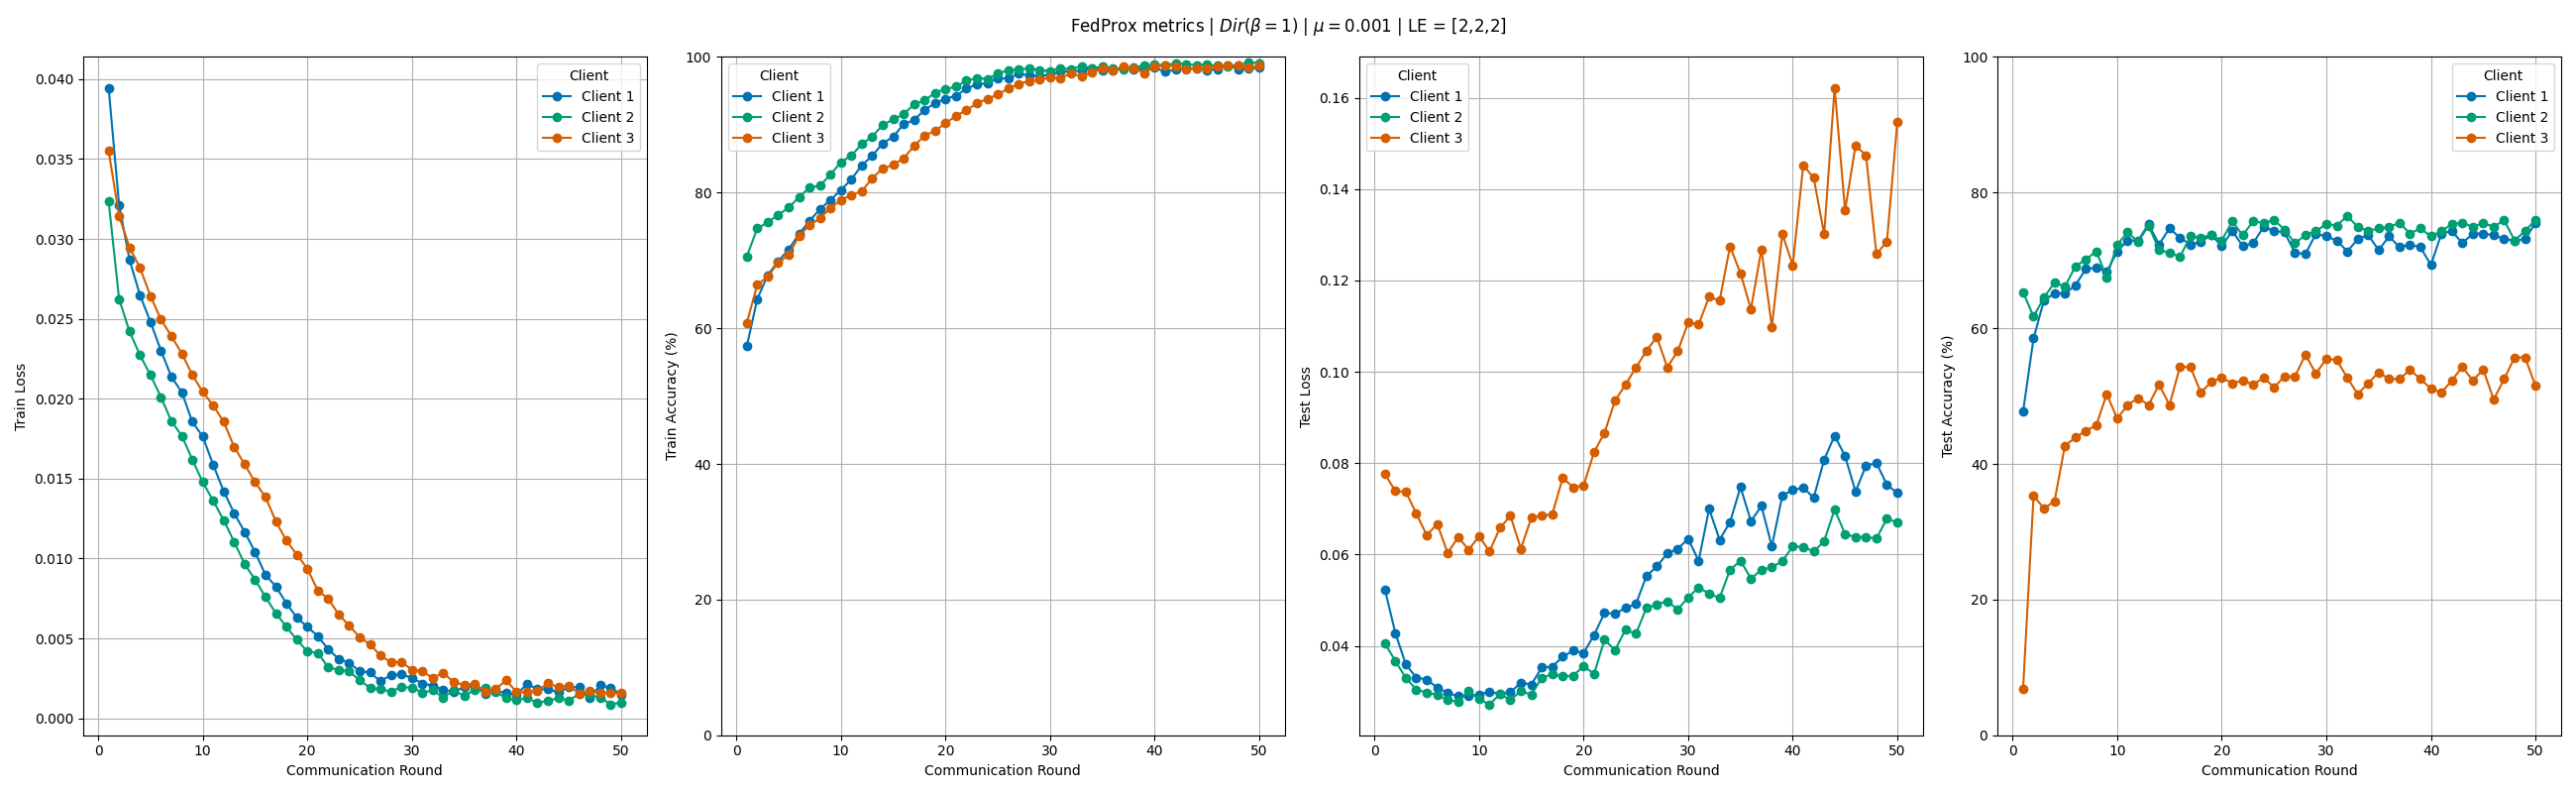
\includegraphics[width=0.8\linewidth]{figures/2-Federated_Learning/FedProx_Dirichlet_1_mu_0.001.png}
    \end{subfigure}
    \vspace{1em} % Space between images

    \begin{subfigure}{\linewidth}
        \centering
        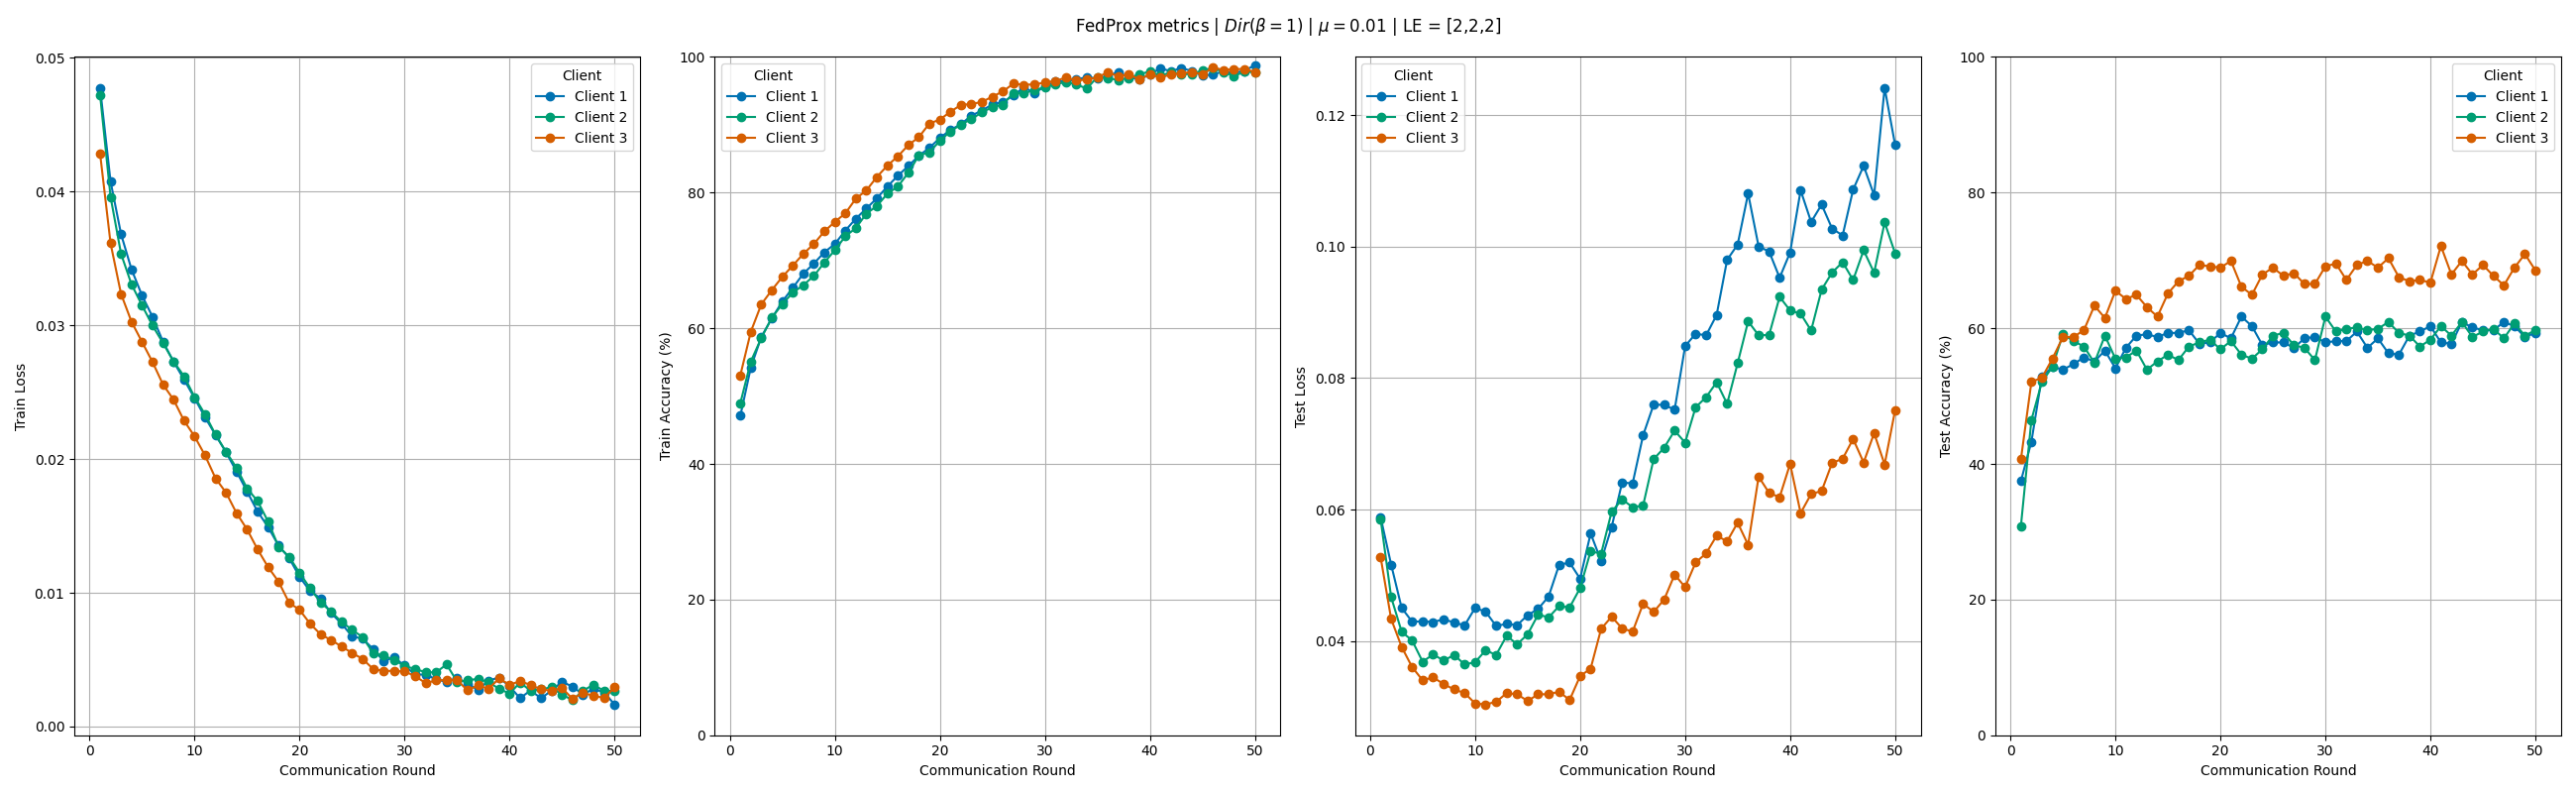
\includegraphics[width=0.8\linewidth]{figures/2-Federated_Learning/FedProx_Dirichlet_1_mu_0.01.png}
    \end{subfigure}
    \vspace{1em} % Space between images

    \begin{subfigure}{\linewidth}
        \centering
        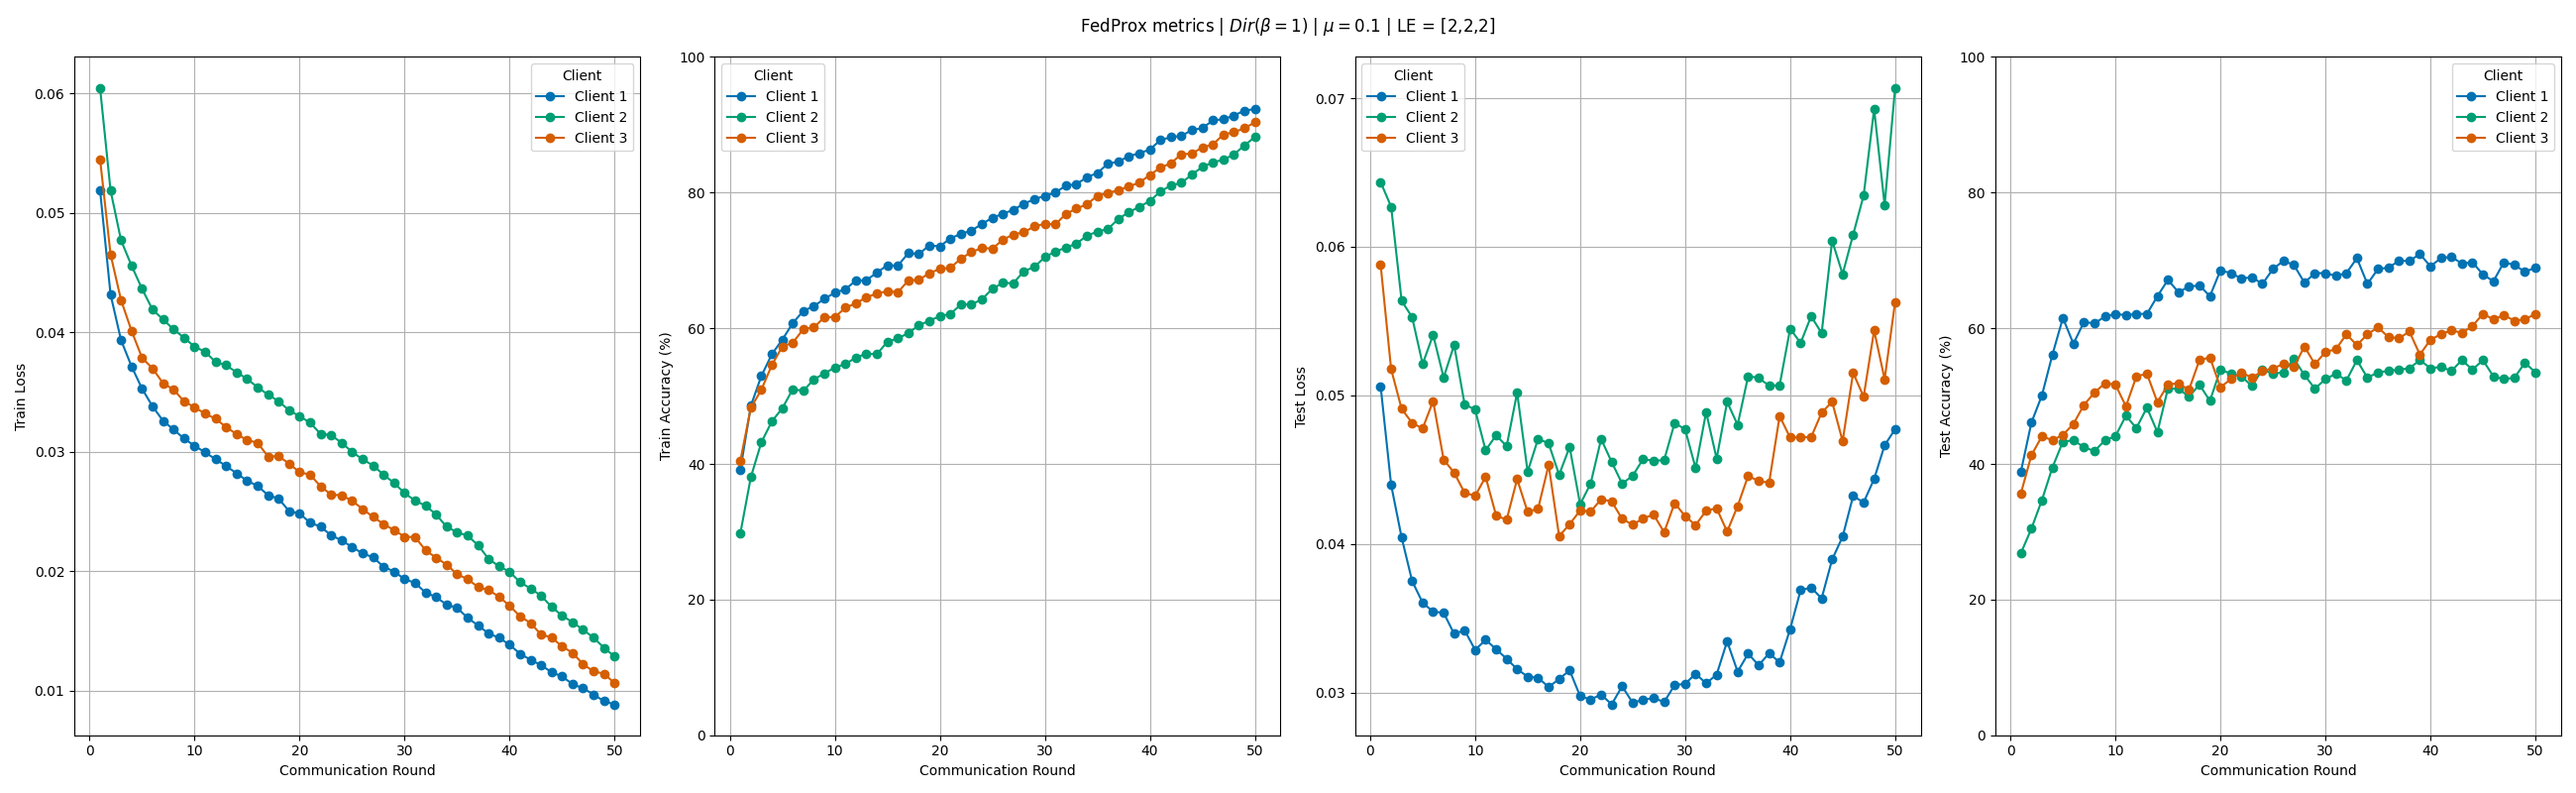
\includegraphics[width=0.8\linewidth]{figures/2-Federated_Learning/FedProx_Dirichlet_1_mu_0.1.png}
    \end{subfigure}
    \vspace{1em} % Space between images

    \begin{subfigure}{\linewidth}
        \centering
        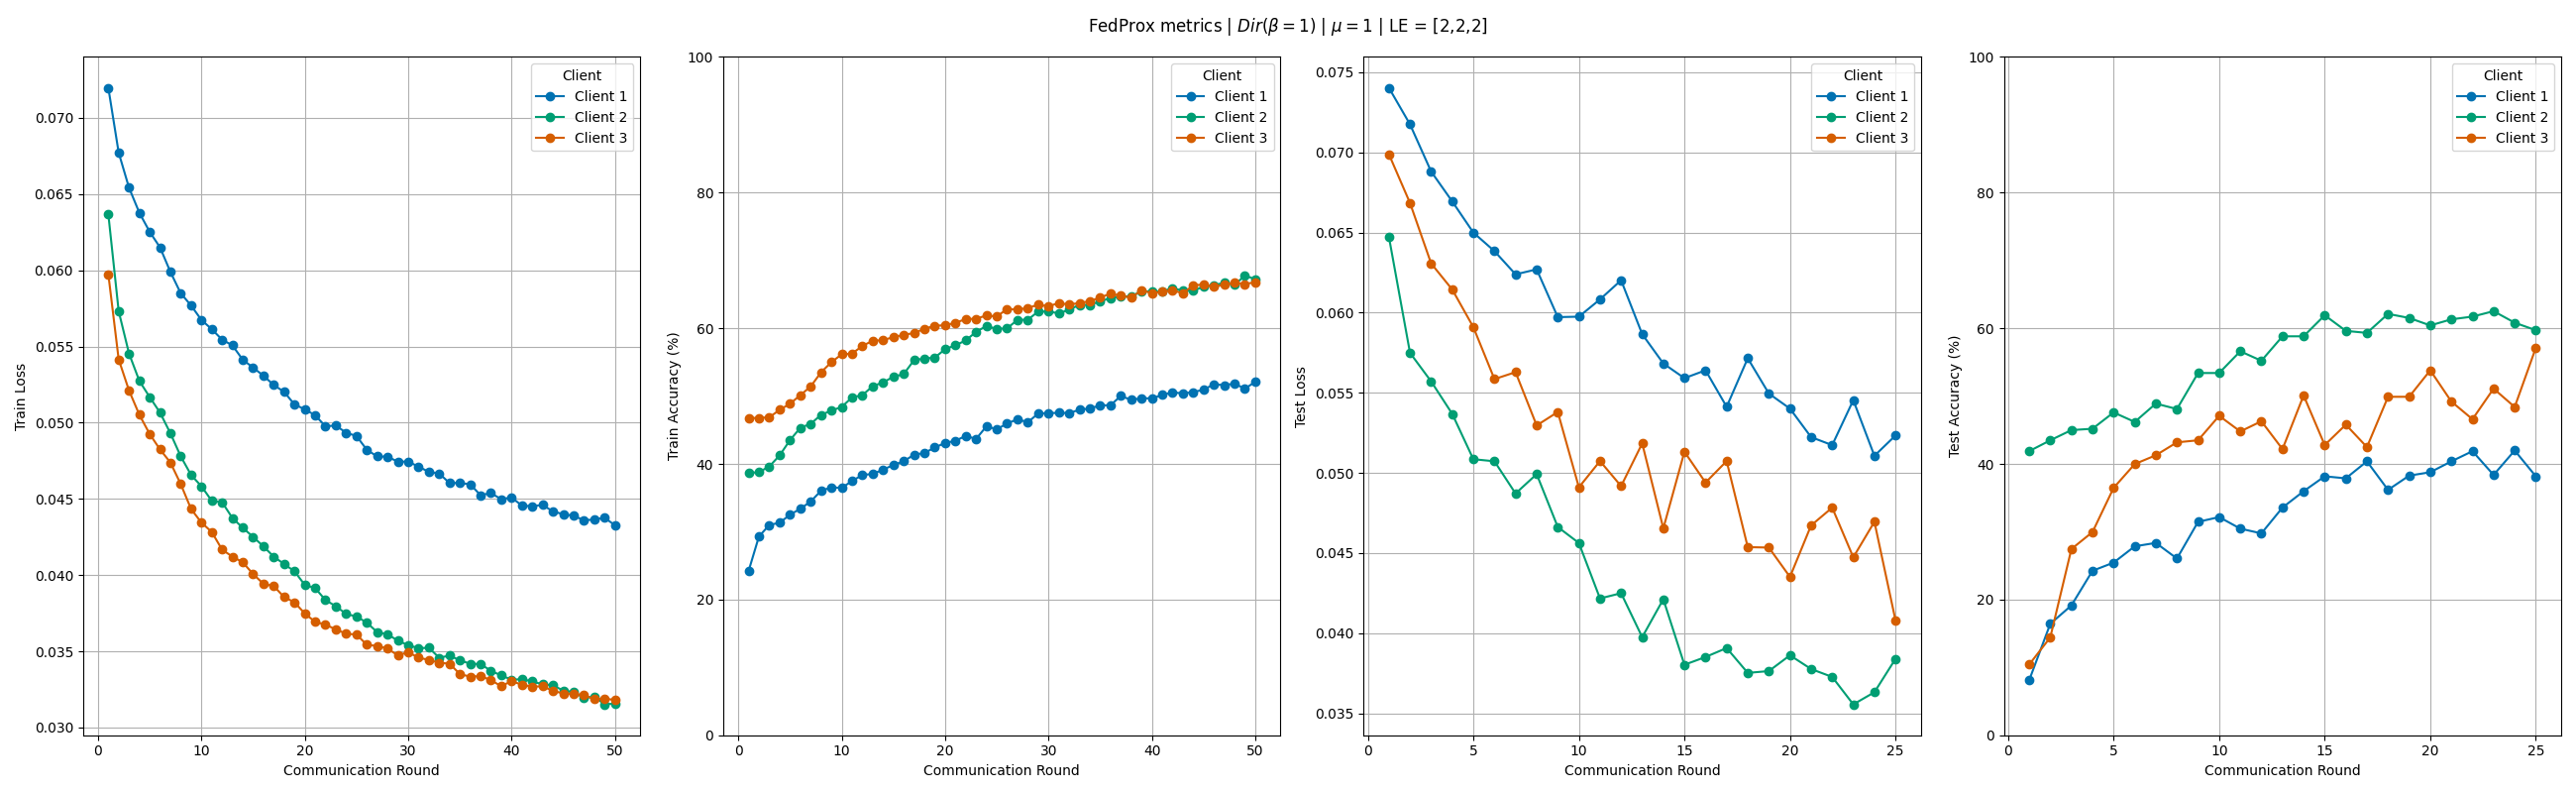
\includegraphics[width=0.8\linewidth]{figures/2-Federated_Learning/FedProx_Dirichlet_1_mu_1.png}
    \end{subfigure}

    \caption{Local metrics for 3 clients in 50 communication rounds using FedProx with a Non-IID setting over the CIFAR10 dataset, $\mu \in \{0.001, 0.01, 0.1, 1\}$. Label distribution skew using the Dirichlet distribution with $\boldsymbol{\beta} = (1,1,1)$ }
    \label{fig:FedProx_Non_IID_Dirichlet_1}
\end{figure}


\begin{figure}[H]
    \centering

    \begin{subfigure}{\linewidth}
        \centering
        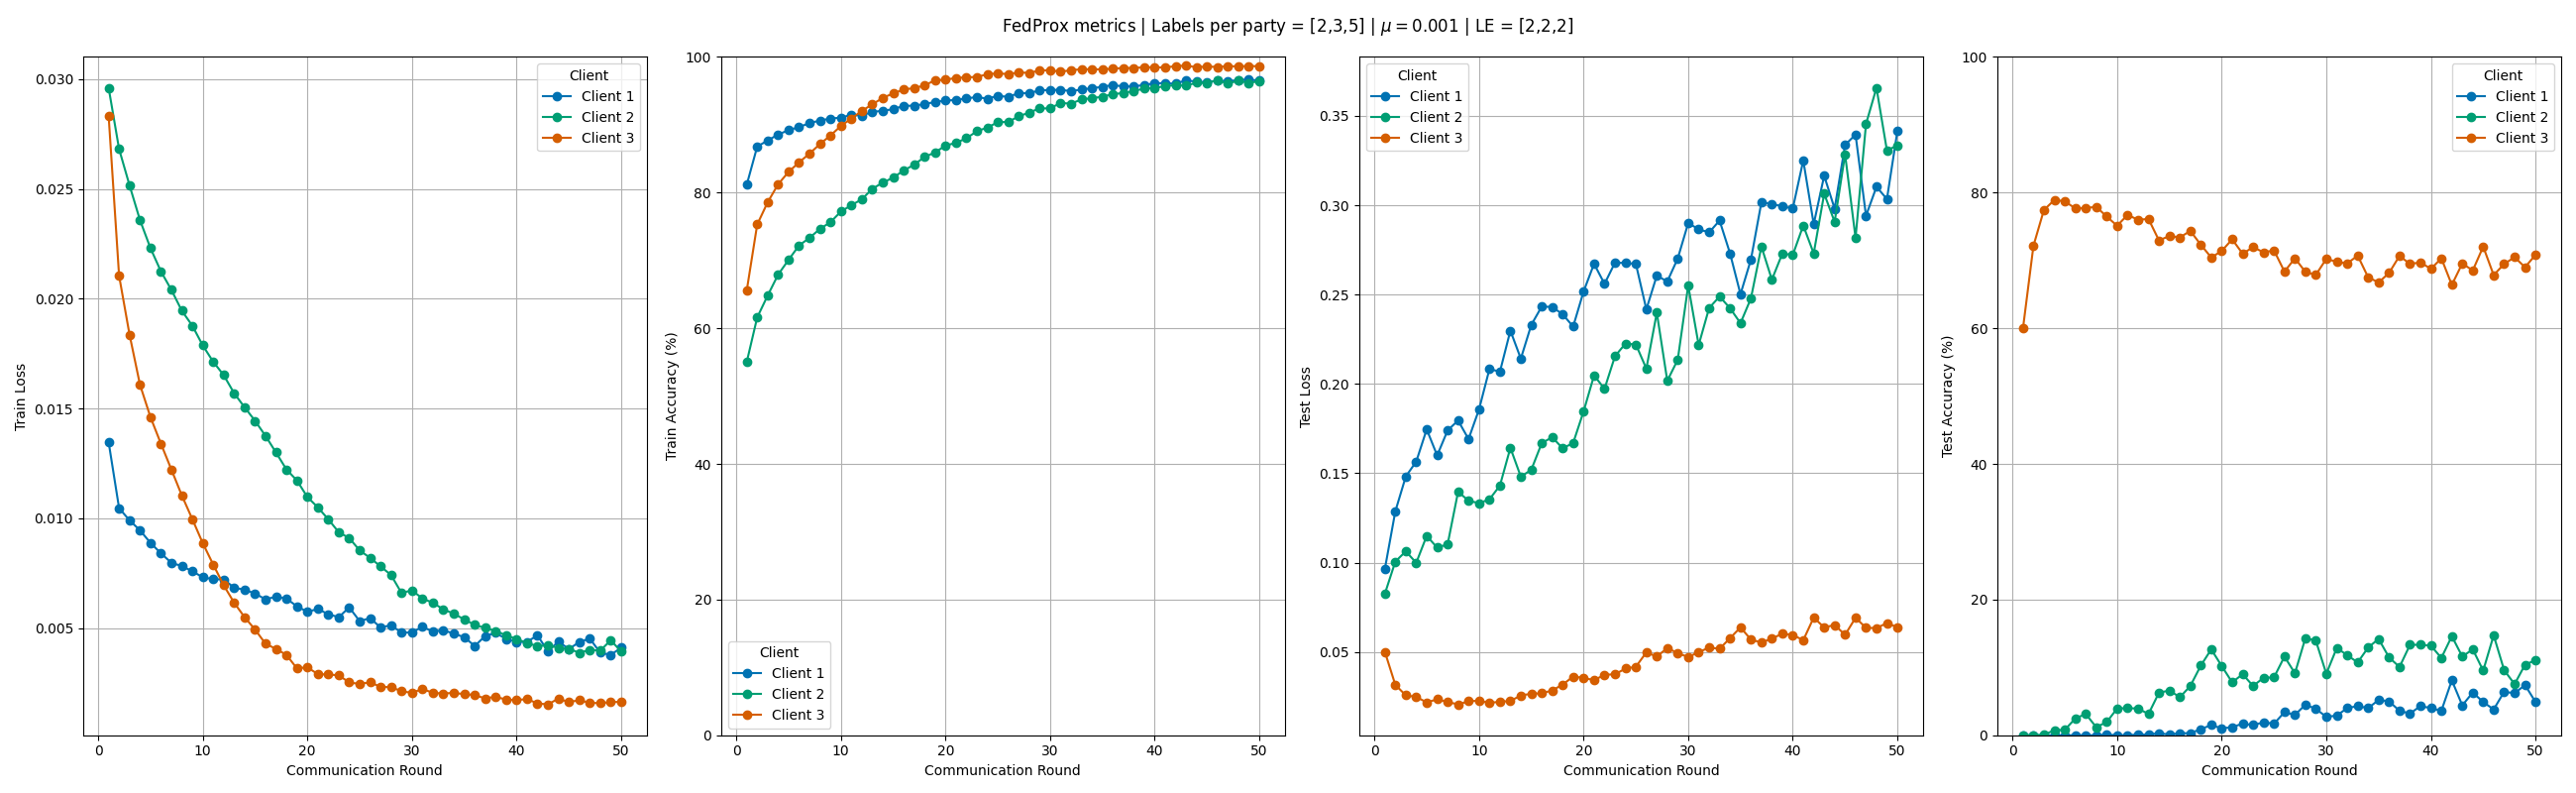
\includegraphics[width=0.8\linewidth]{figures/2-Federated_Learning/FedProx_LabelsPerParty_mu_0.001.png}
    \end{subfigure}
    \vspace{1em} % Space between images

    \begin{subfigure}{\linewidth}
        \centering
        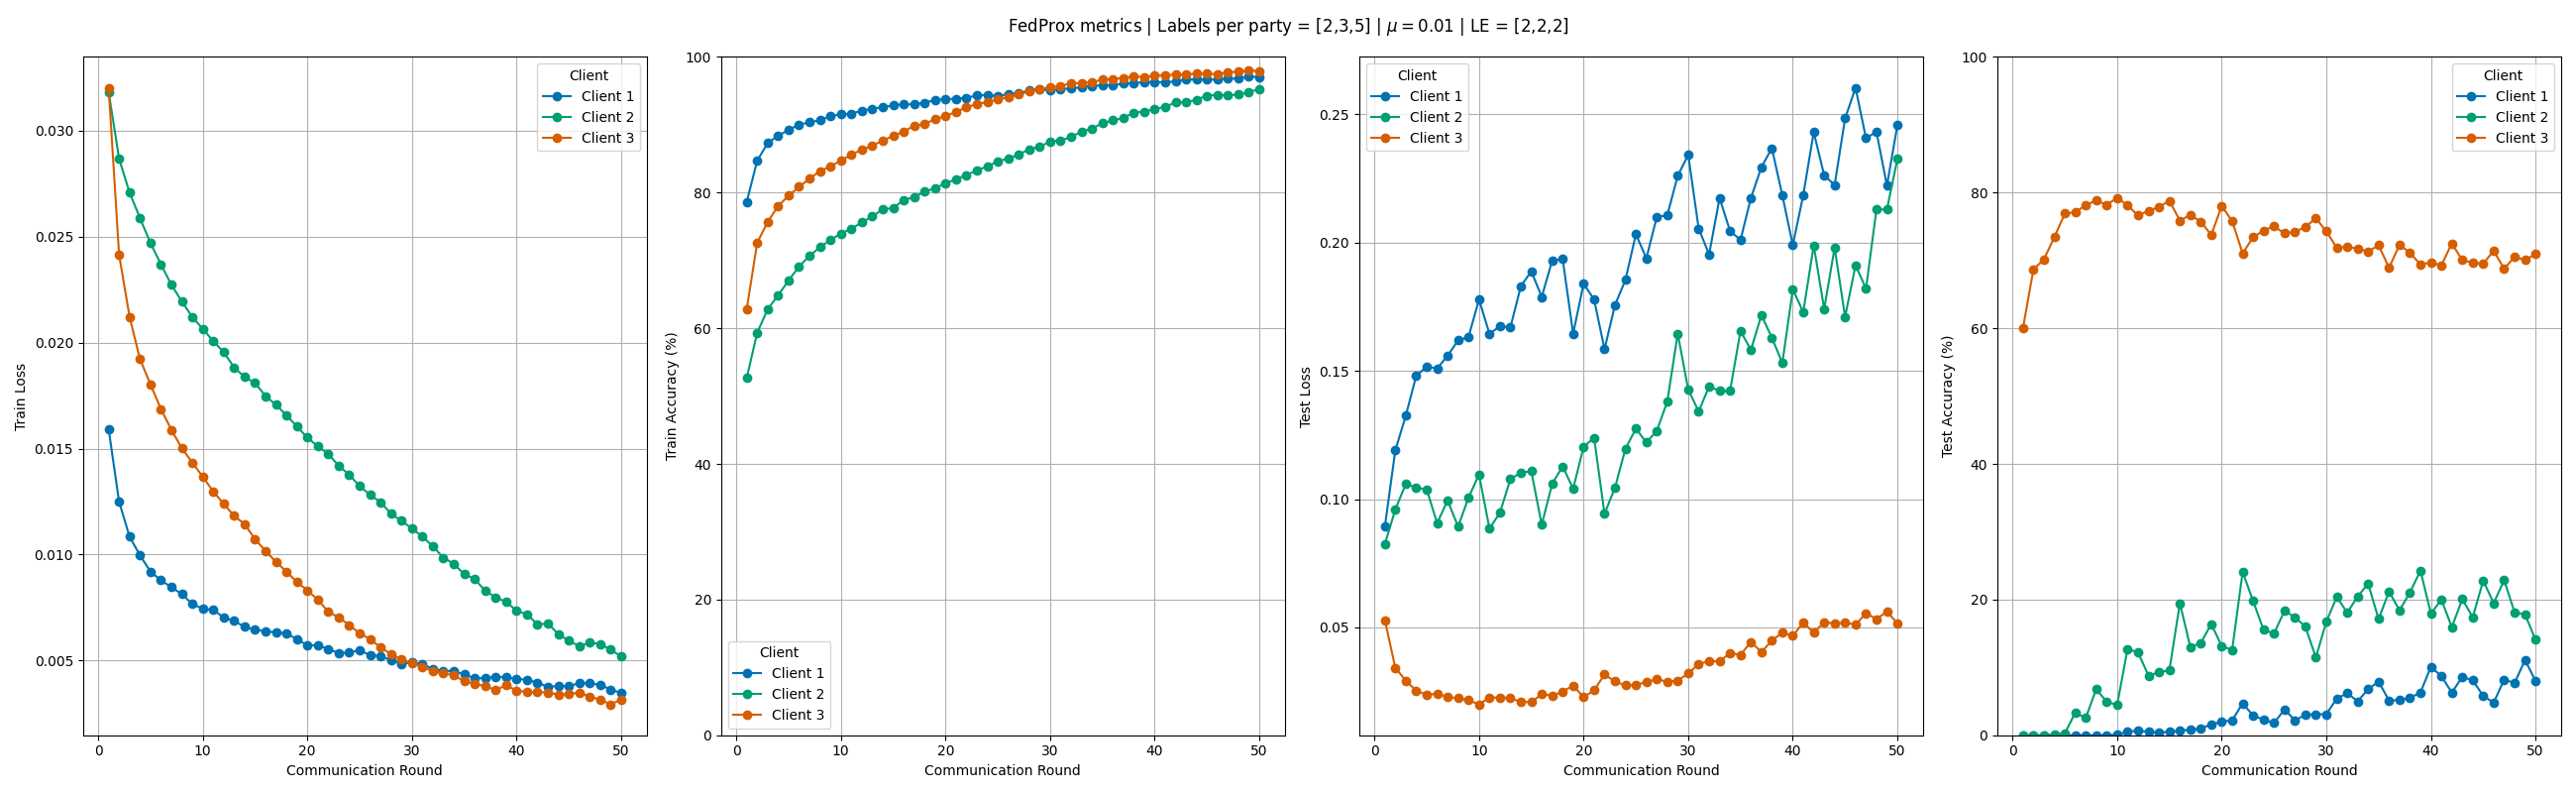
\includegraphics[width=0.8\linewidth]{figures/2-Federated_Learning/FedProx_LabelsPerParty_mu_0.01.png}
    \end{subfigure}
    \vspace{1em} % Space between images

    \begin{subfigure}{\linewidth}
        \centering
        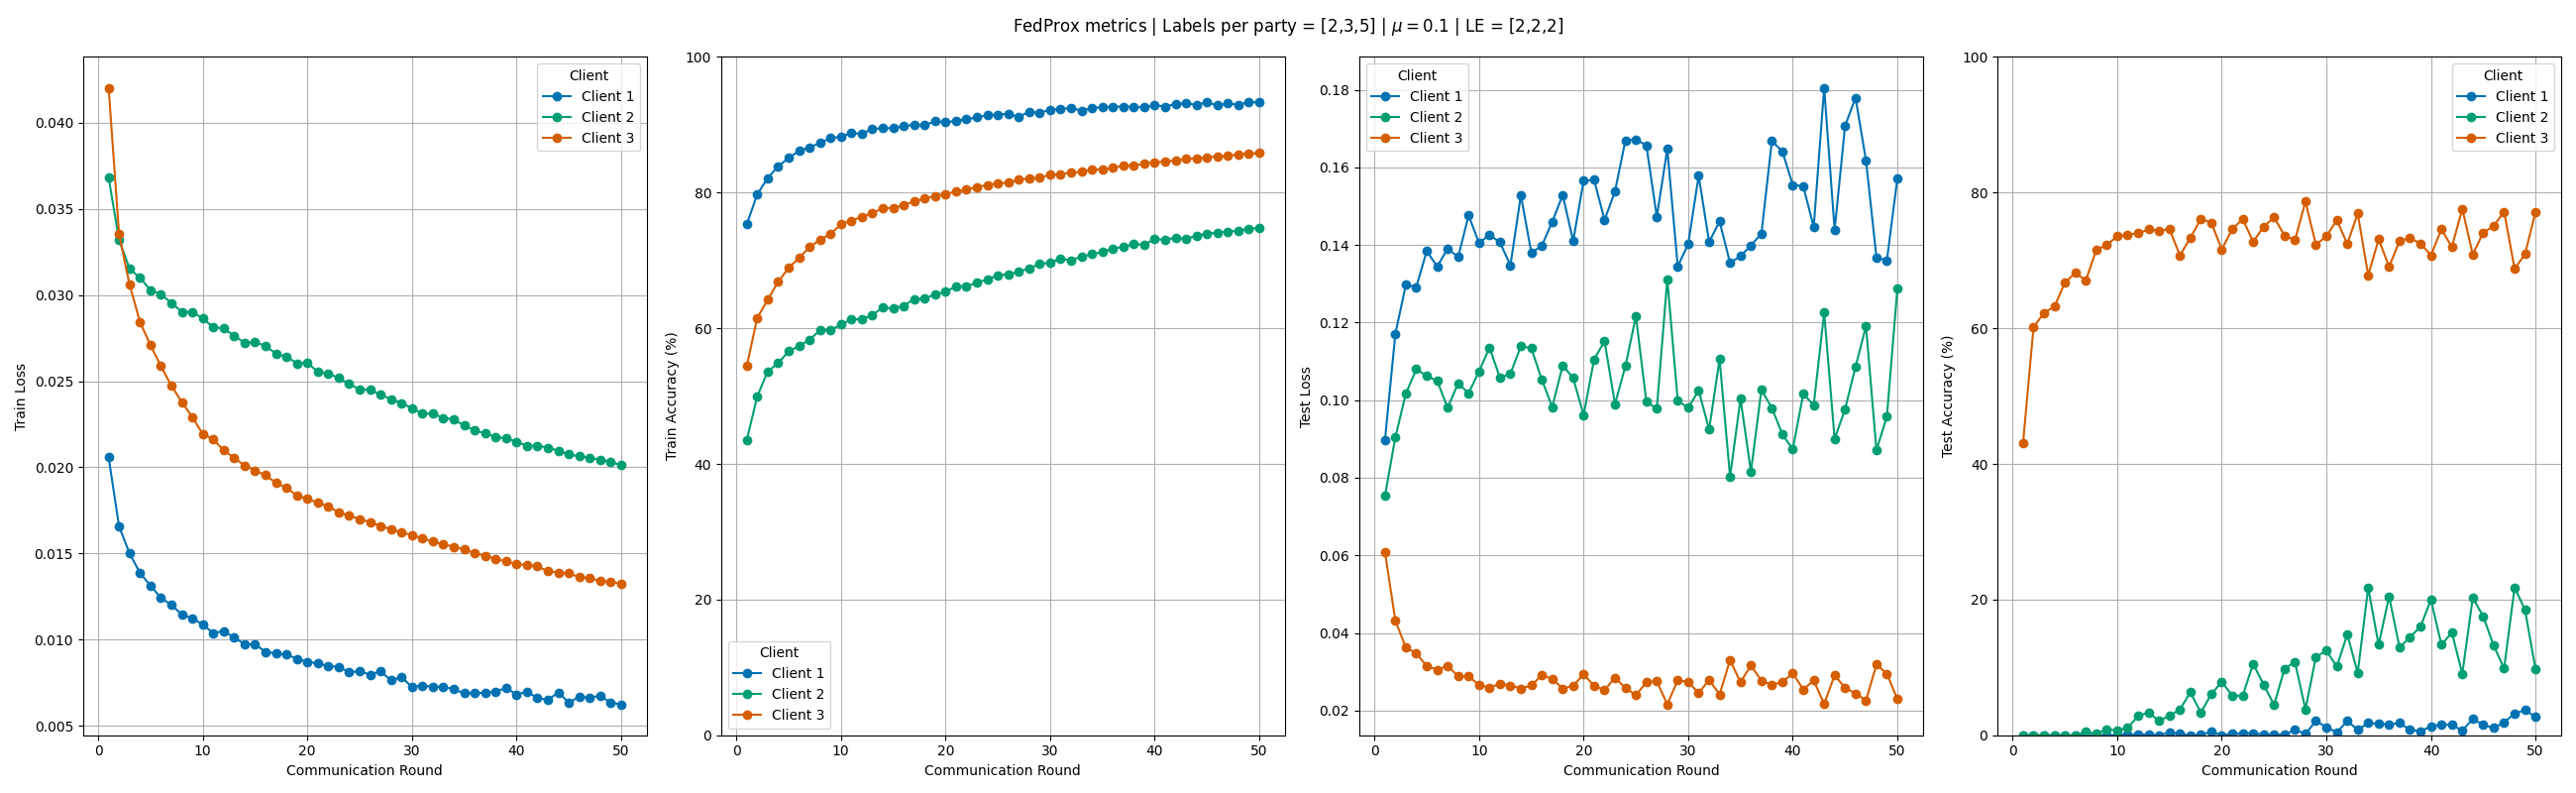
\includegraphics[width=0.8\linewidth]{figures/2-Federated_Learning/FedProx_LabelsPerParty_mu_0.1.png}
    \end{subfigure}
    \vspace{1em} % Space between images

    \begin{subfigure}{\linewidth}
        \centering
        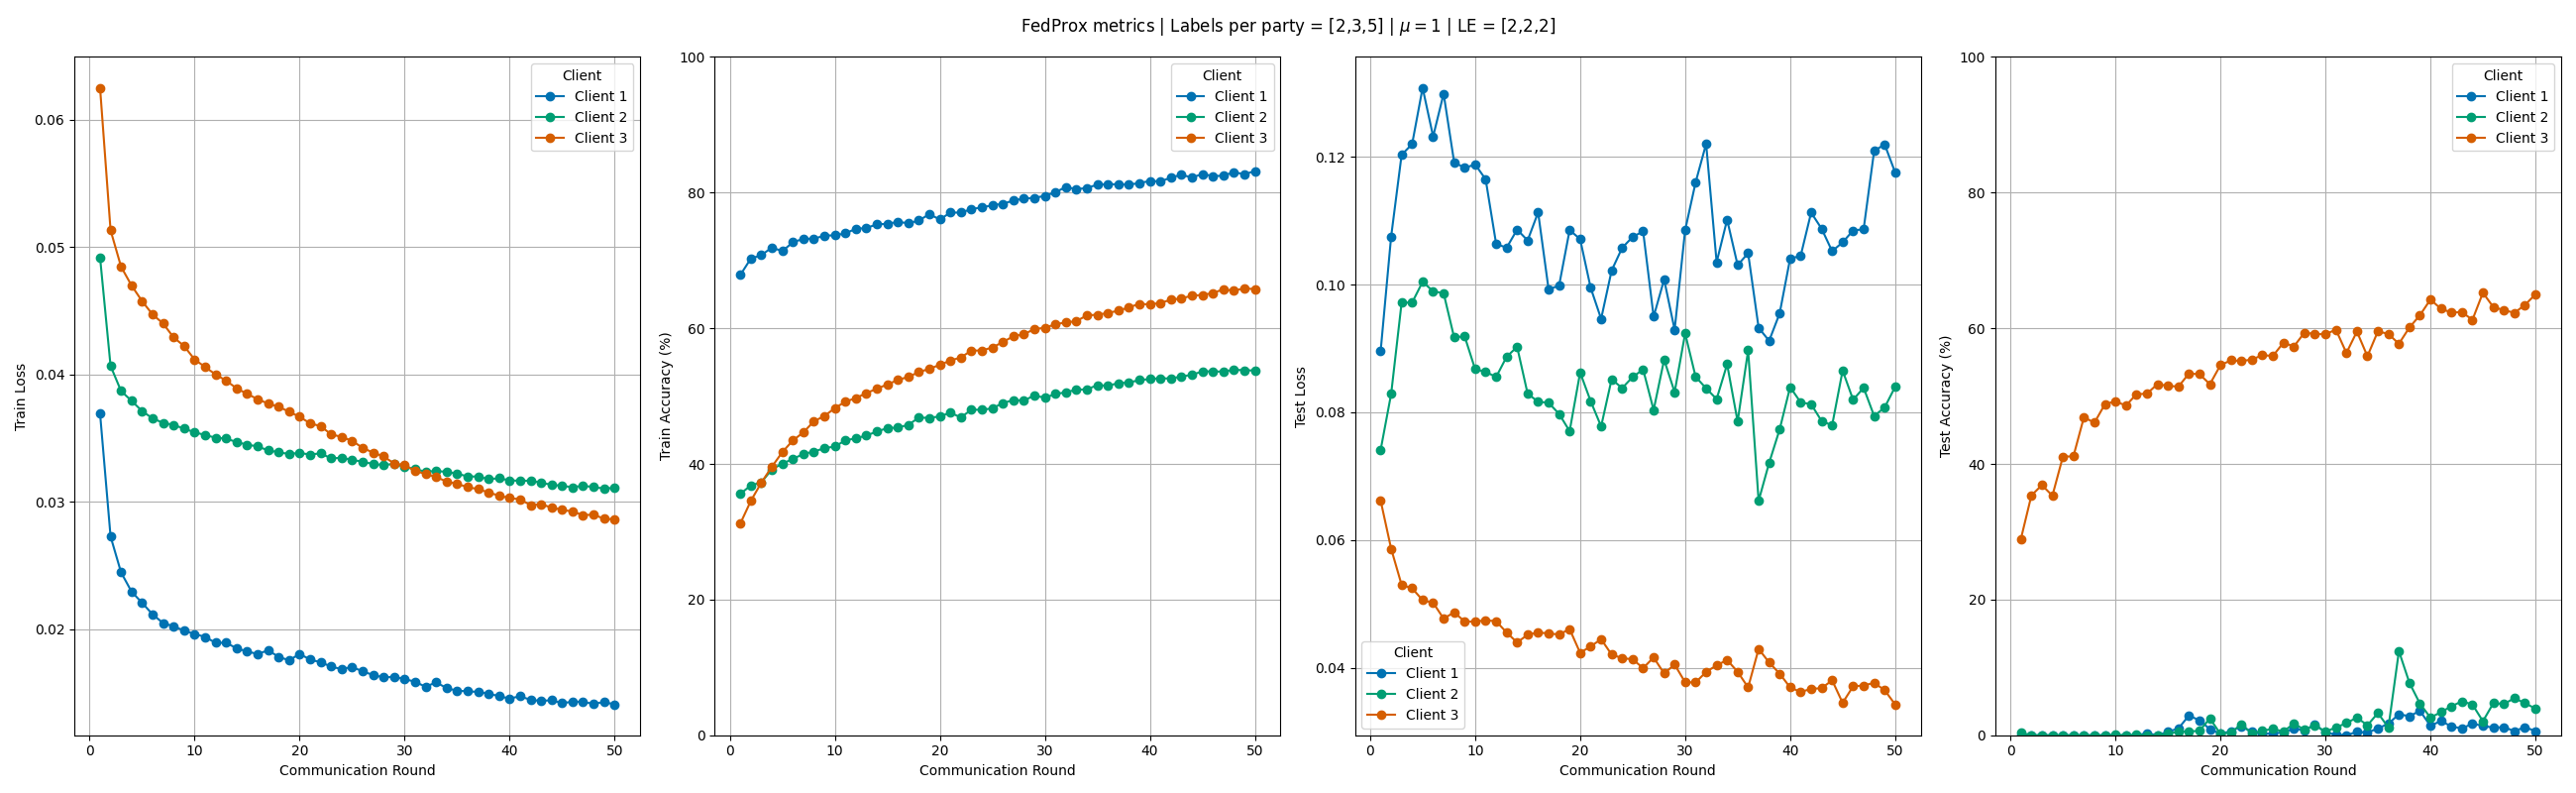
\includegraphics[width=0.8\linewidth]{figures/2-Federated_Learning/FedProx_LabelsPerParty_mu_1.png}
    \end{subfigure}

    \caption{Local metrics for 3 clients in 50 communication rounds using FedProx with a Non-IID setting over the CIFAR10 dataset, $\mu \in \{0.001, 0.01, 0.1, 1\}$.  Label distribution skew, the first client data from 2 classes, the second client
from 3 classes and the third client from the 5 remaining classes.}
    \label{fig:FedProx_Non_IID_LabelsPerParty}
\end{figure}




\begin{figure}[H]
    \centering

    \begin{subfigure}{\linewidth}
        \centering
        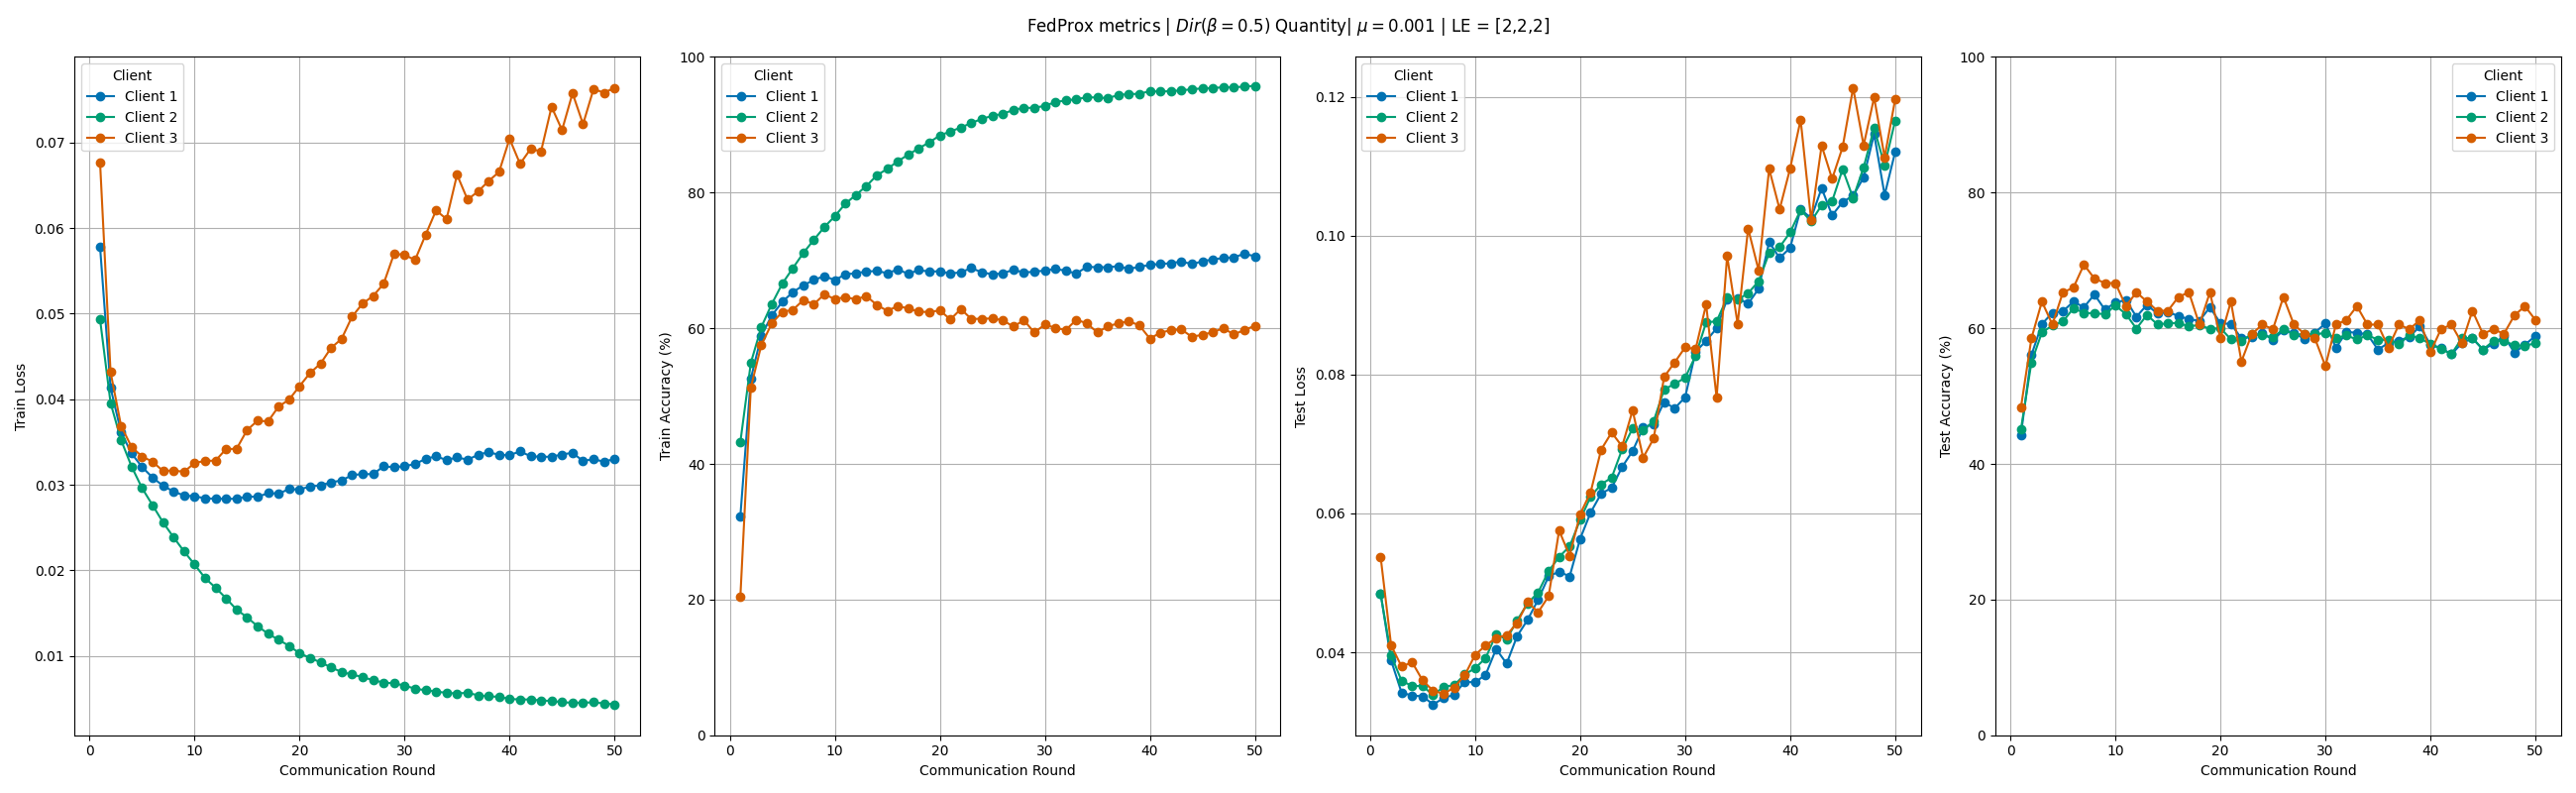
\includegraphics[width=0.8\linewidth]{figures/2-Federated_Learning/FedProx_QuantitySkew_Dir_05_Mu_0.001.png}
    \end{subfigure}
    \vspace{1em} % Space between images

    \begin{subfigure}{\linewidth}
        \centering
        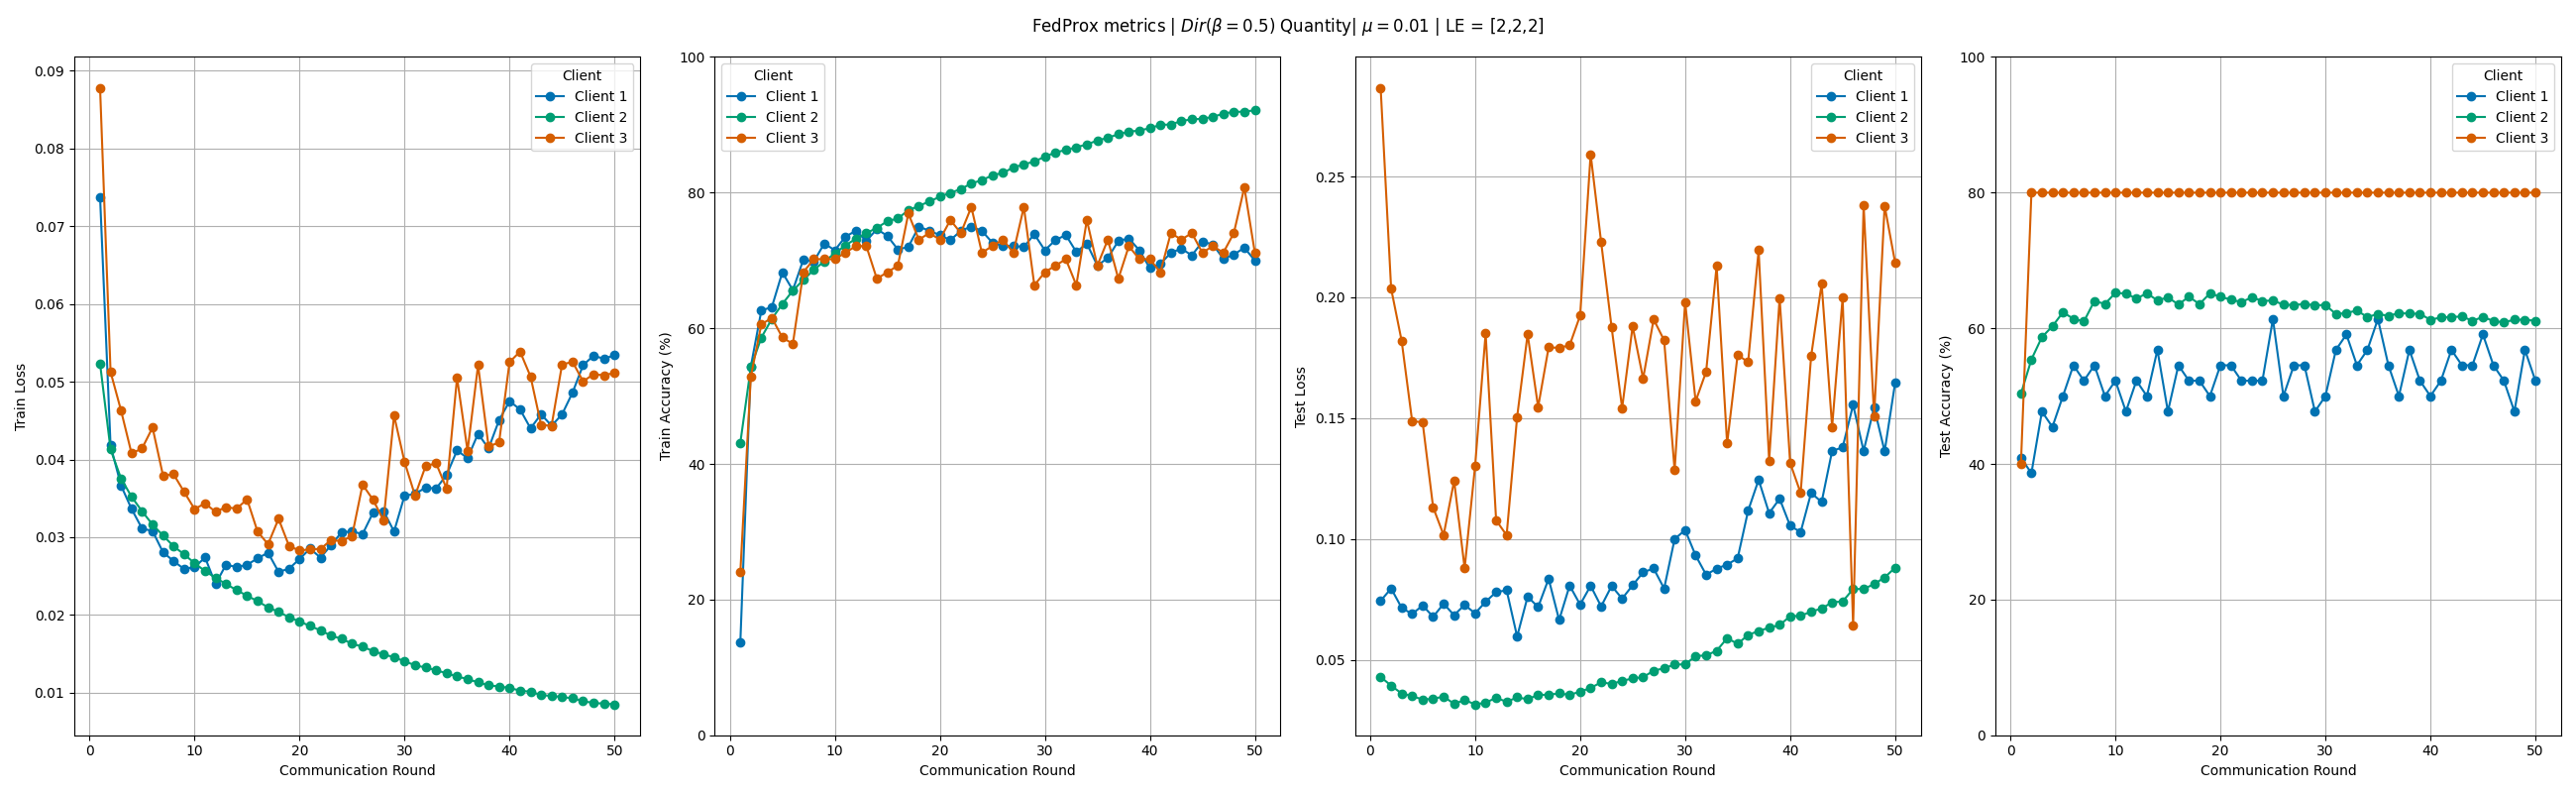
\includegraphics[width=0.8\linewidth]{figures/2-Federated_Learning/FedProx_QuantitySkew_Dir_05_Mu_0.01.png}
    \end{subfigure}
    \vspace{1em} % Space between images

    \begin{subfigure}{\linewidth}
        \centering
        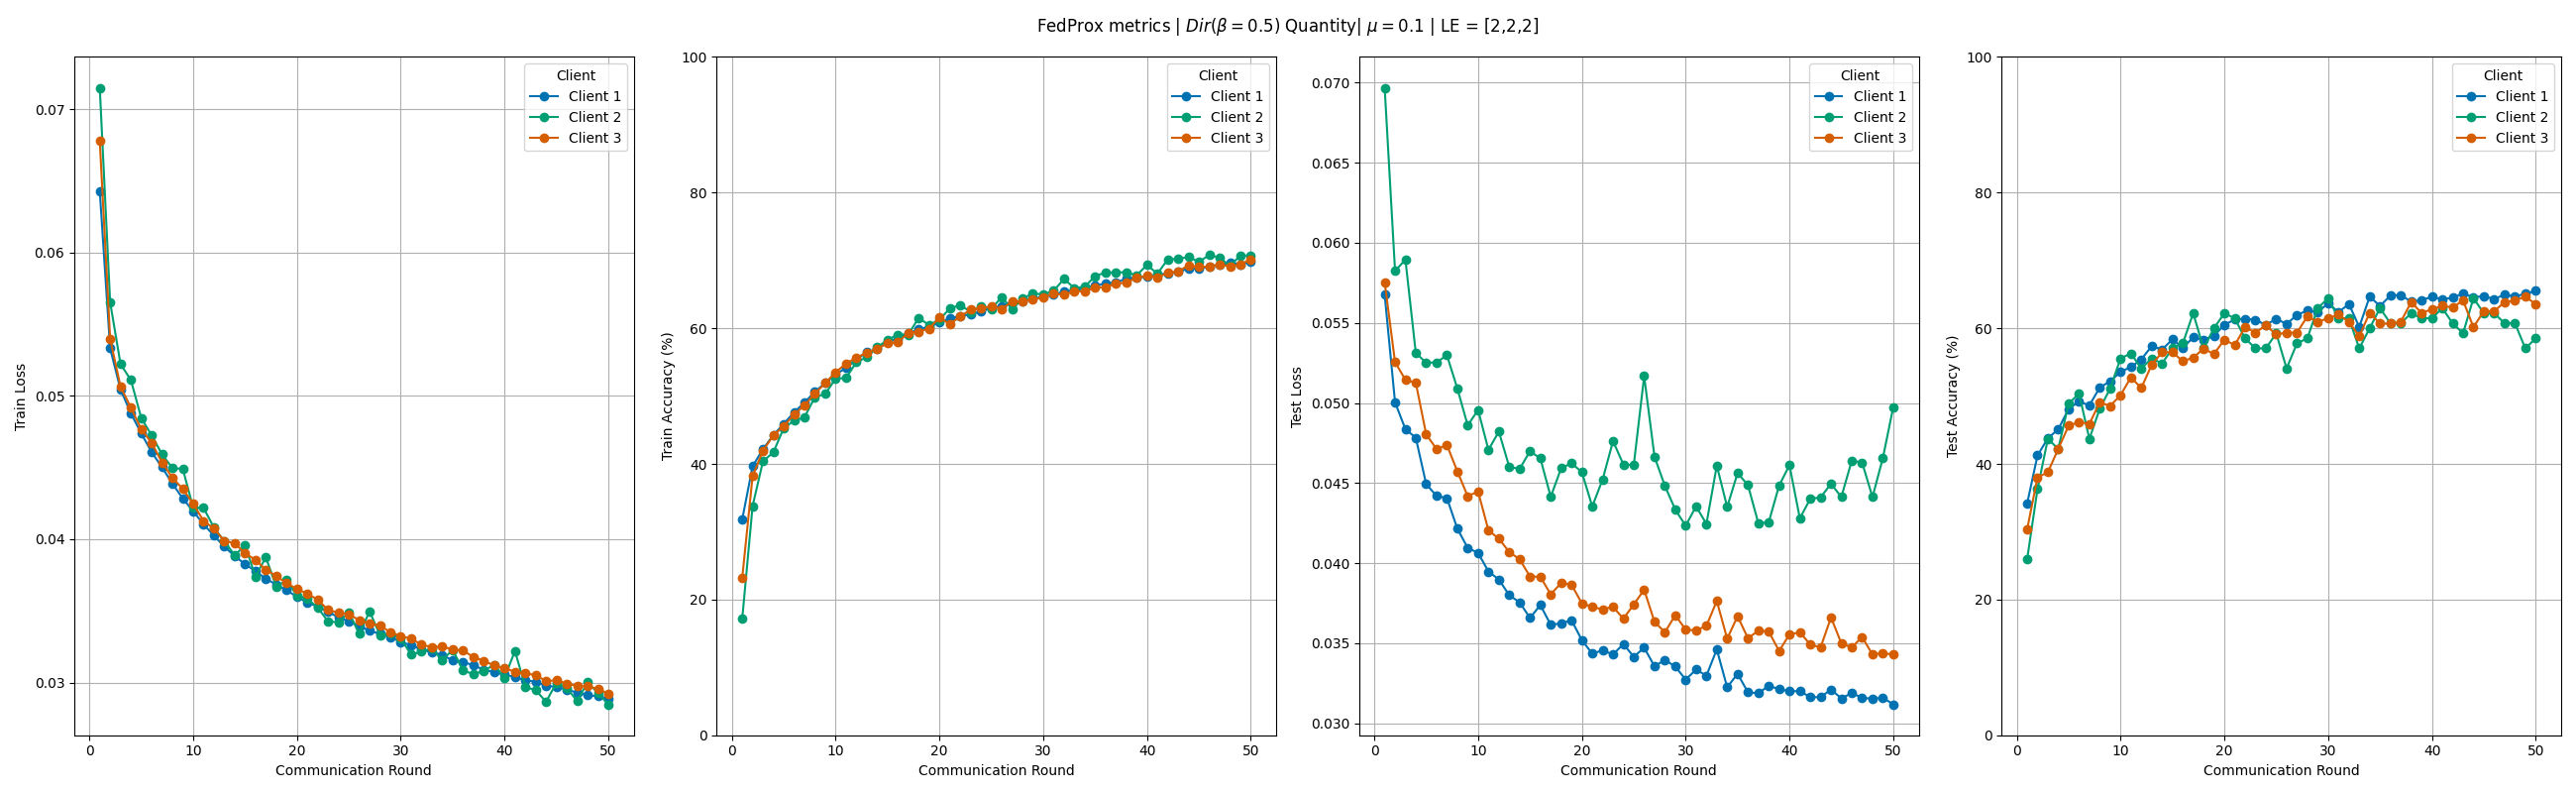
\includegraphics[width=0.8\linewidth]{figures/2-Federated_Learning/FedProx_QuantitySkew_Dir_05_Mu_0.1.png}
    \end{subfigure}
    \vspace{1em} % Space between images

    \begin{subfigure}{\linewidth}
        \centering
        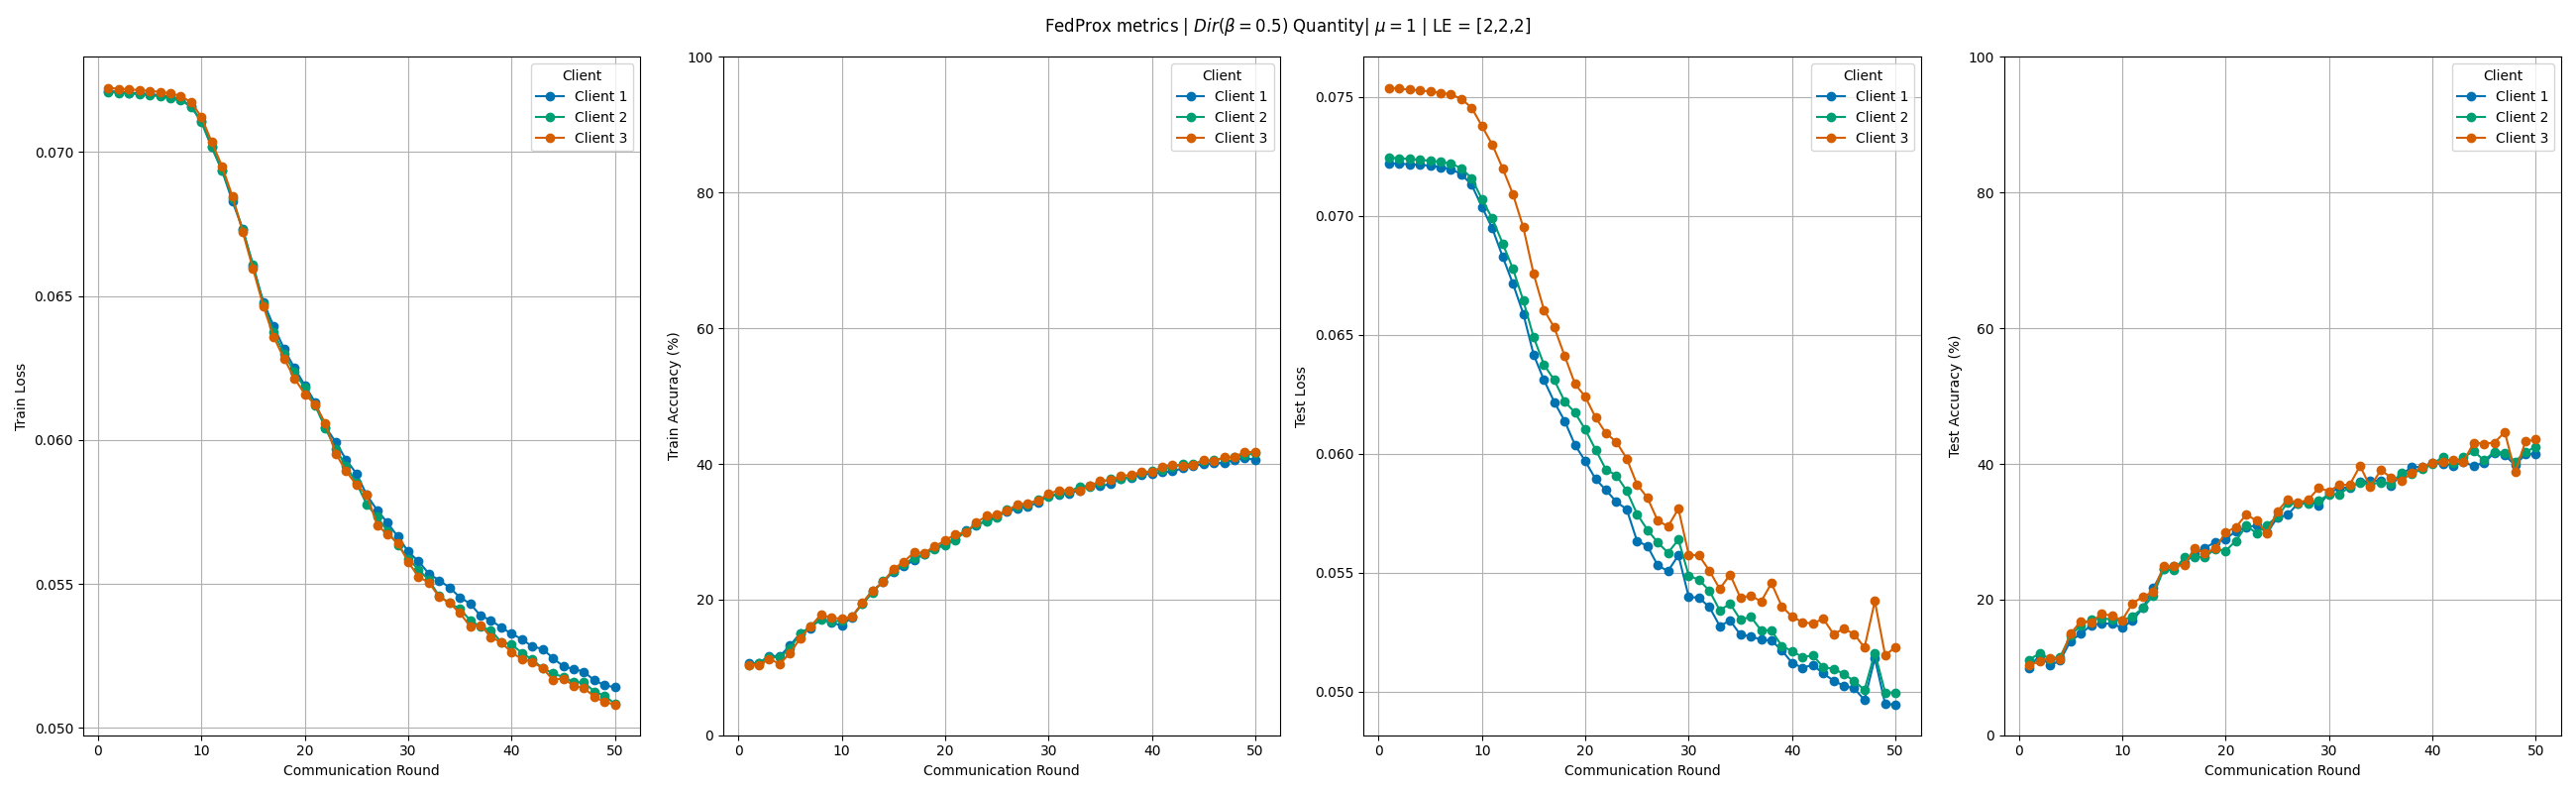
\includegraphics[width=0.8\linewidth]{figures/2-Federated_Learning/FedProx_QuantitySkew_Dir_05_Mu_1.png}
    \end{subfigure}

    \caption{Local metrics for 3 clients in 50 communication rounds using FedProx with a Non-IID setting over the CIFAR10 dataset, $\mu \in \{0.001, 0.01, 0.1, 1\}$.  Label quantity distribution skew using $Dir(\boldsymbol{\beta})$, $\boldsymbol{\beta} = (0.5,0.5,0.5)$  }
    \label{fig:FedProx_Non_IID_LabelQuantitySkeqDir_05}
\end{figure}




\begin{figure}[H]
    \centering

    \begin{subfigure}{\linewidth}
        \centering
        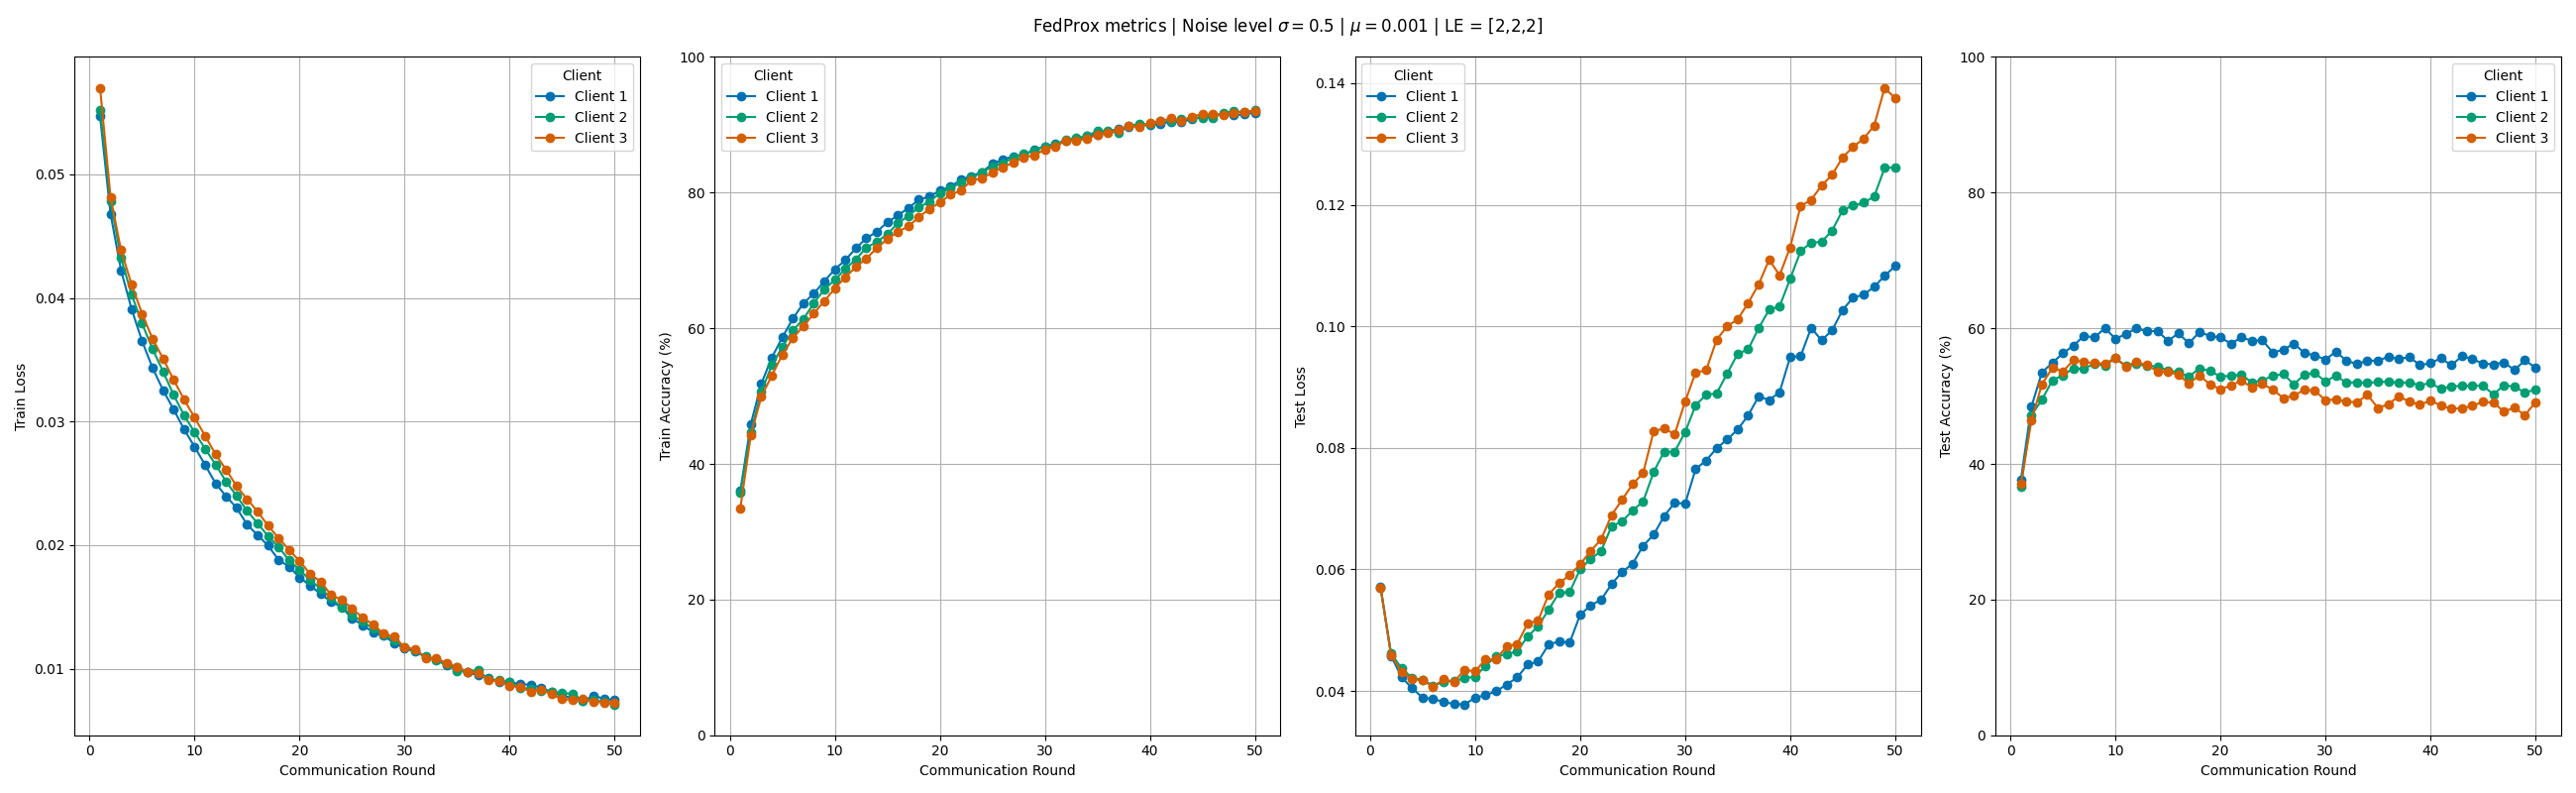
\includegraphics[width=0.8\linewidth]{figures/2-Federated_Learning/FedProx_NoiseLevel_Mu_0.001.png}
    \end{subfigure}
    \vspace{1em} % Space between images

    \begin{subfigure}{\linewidth}
        \centering
        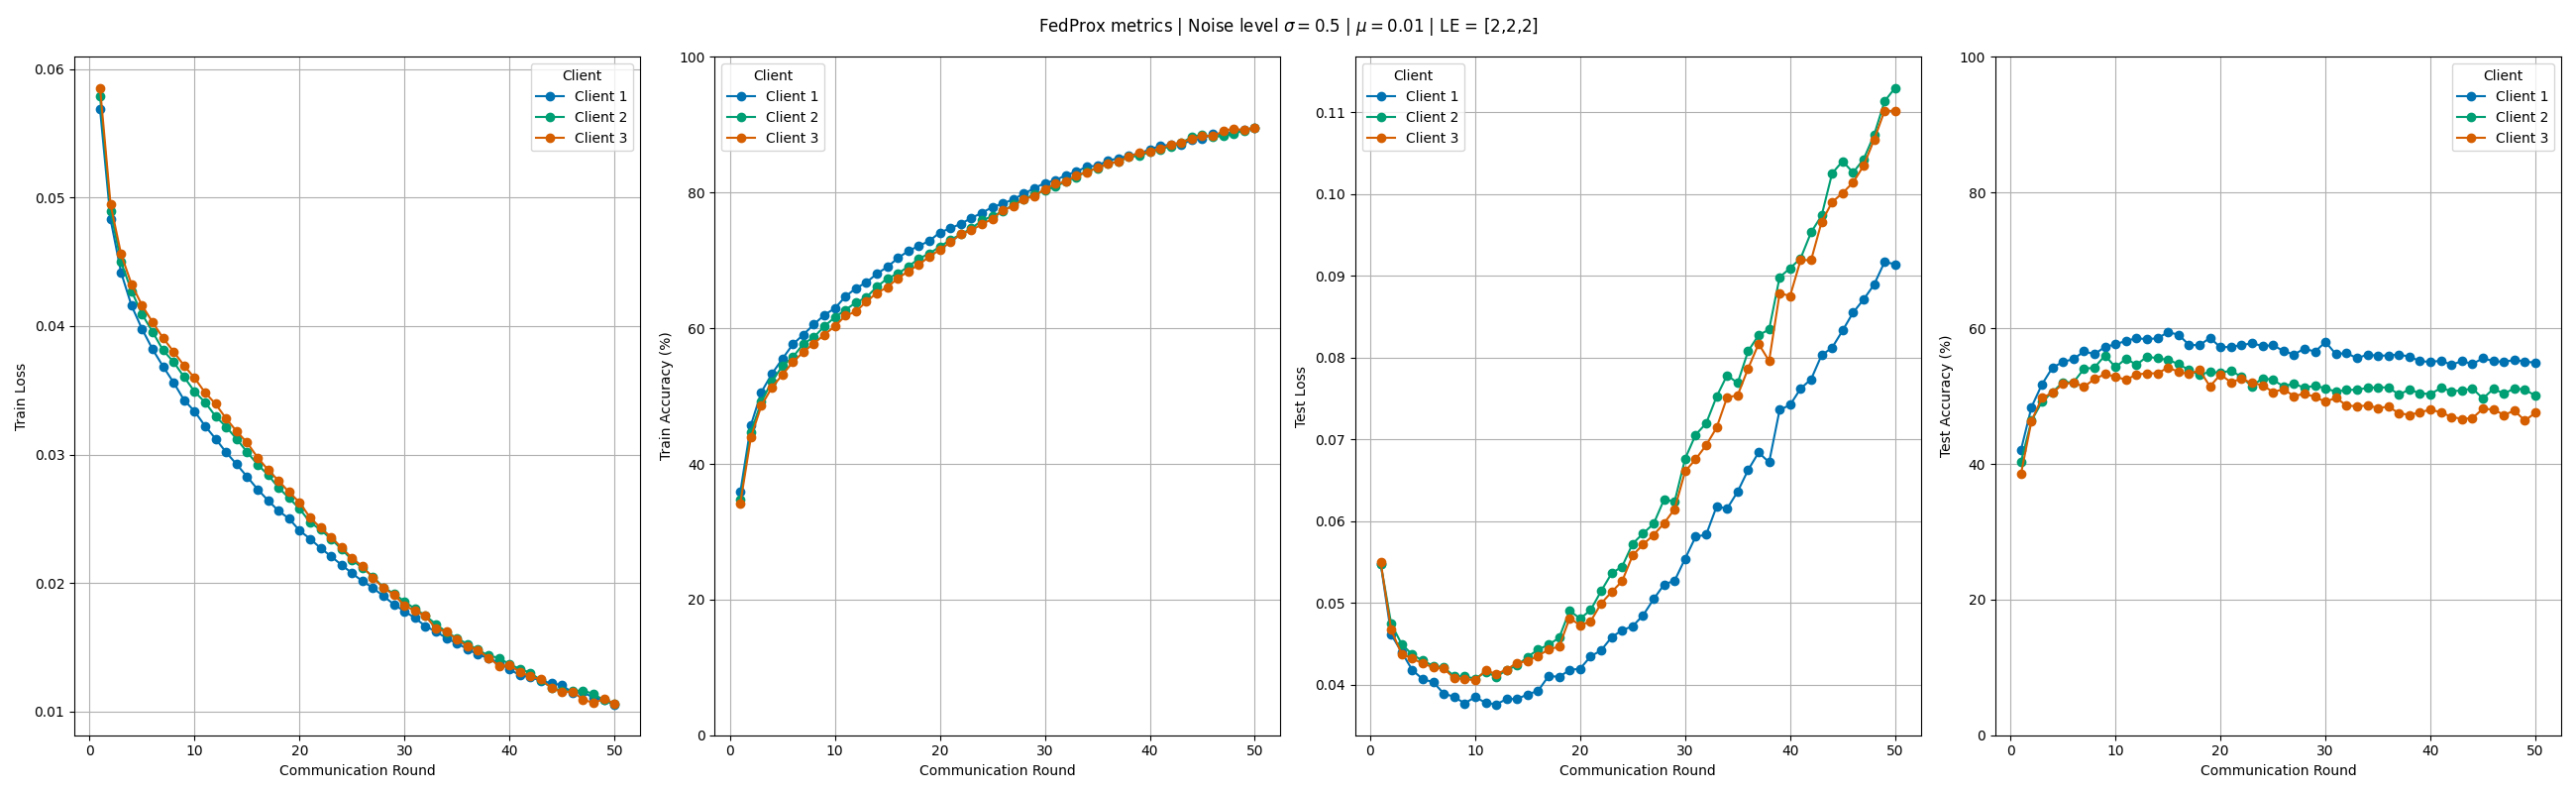
\includegraphics[width=0.8\linewidth]{figures/2-Federated_Learning/FedProx_NoiseLevel_Mu_0.01.png}
    \end{subfigure}
    \vspace{1em} % Space between images

    \begin{subfigure}{\linewidth}
        \centering
        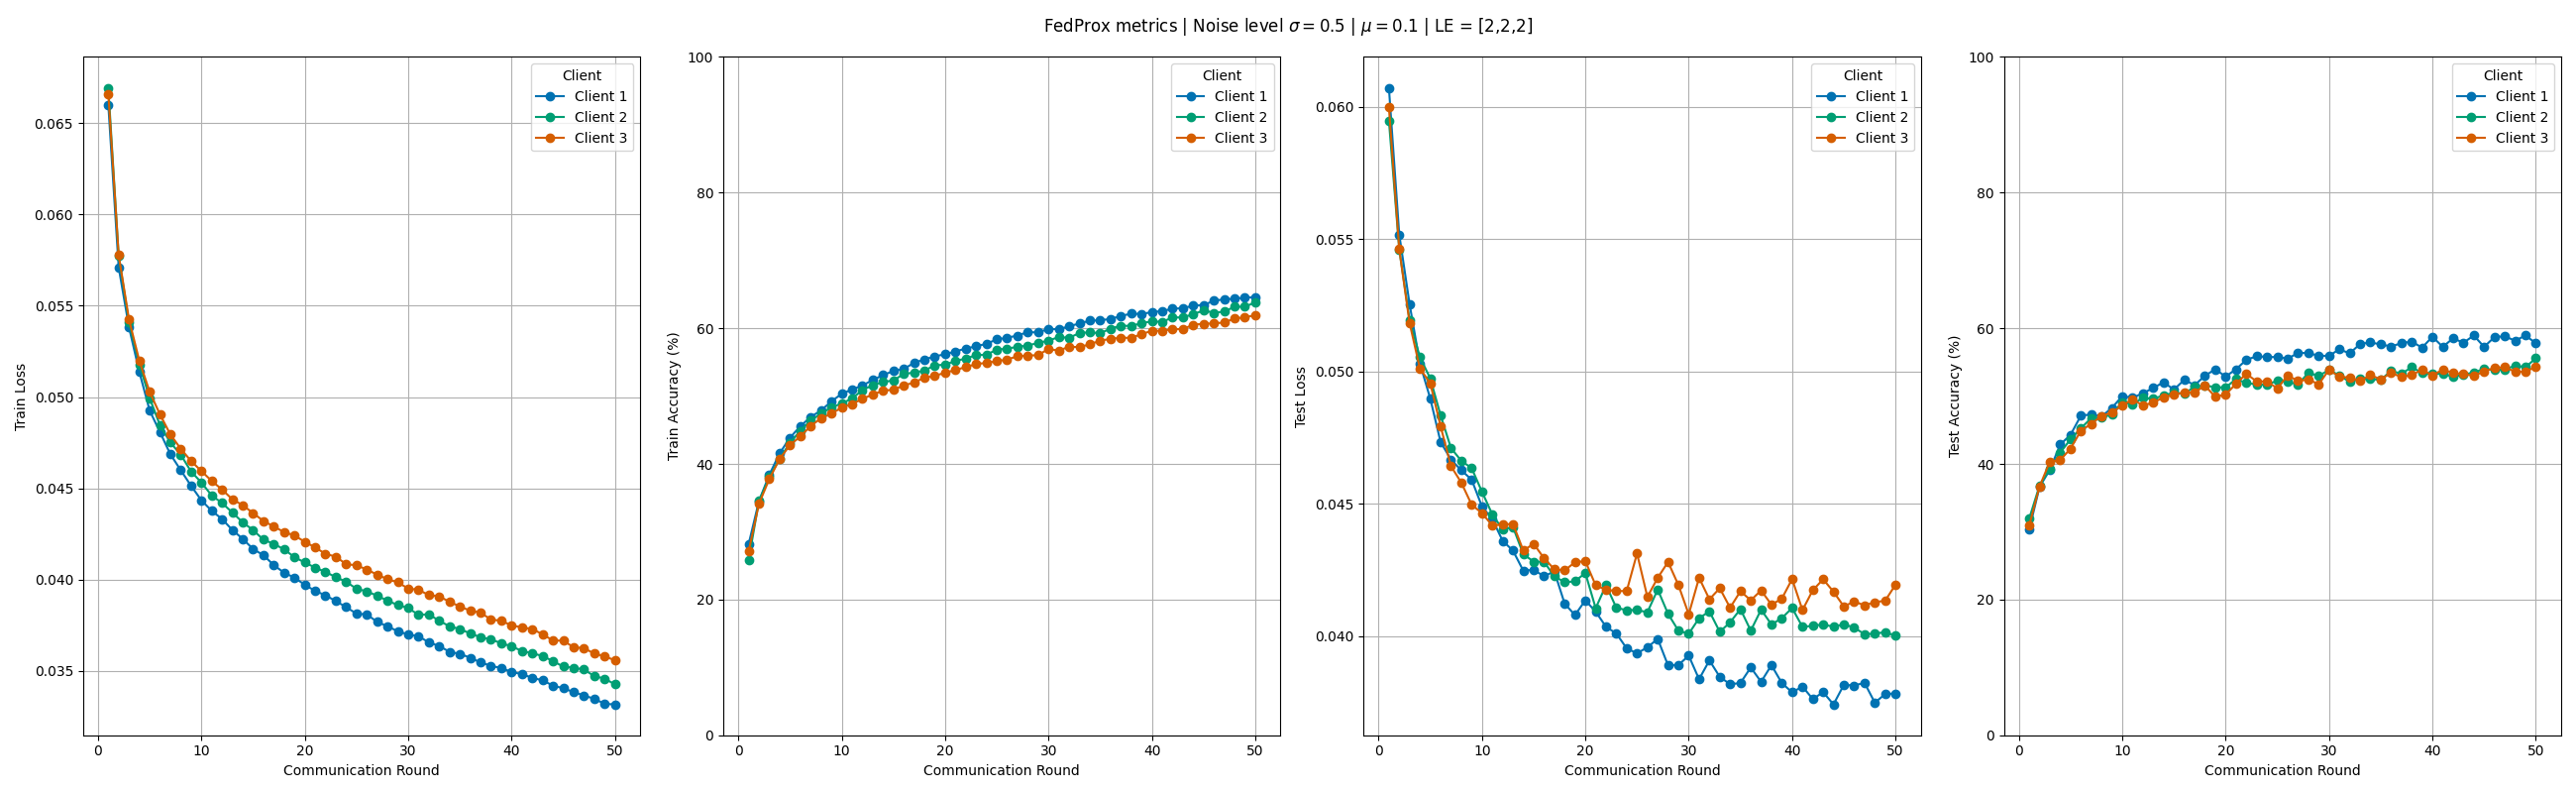
\includegraphics[width=0.8\linewidth]{figures/2-Federated_Learning/FedProx_NoiseLevel_Mu_0.1.png}
    \end{subfigure}
    \vspace{1em} % Space between images

    \begin{subfigure}{\linewidth}
        \centering
        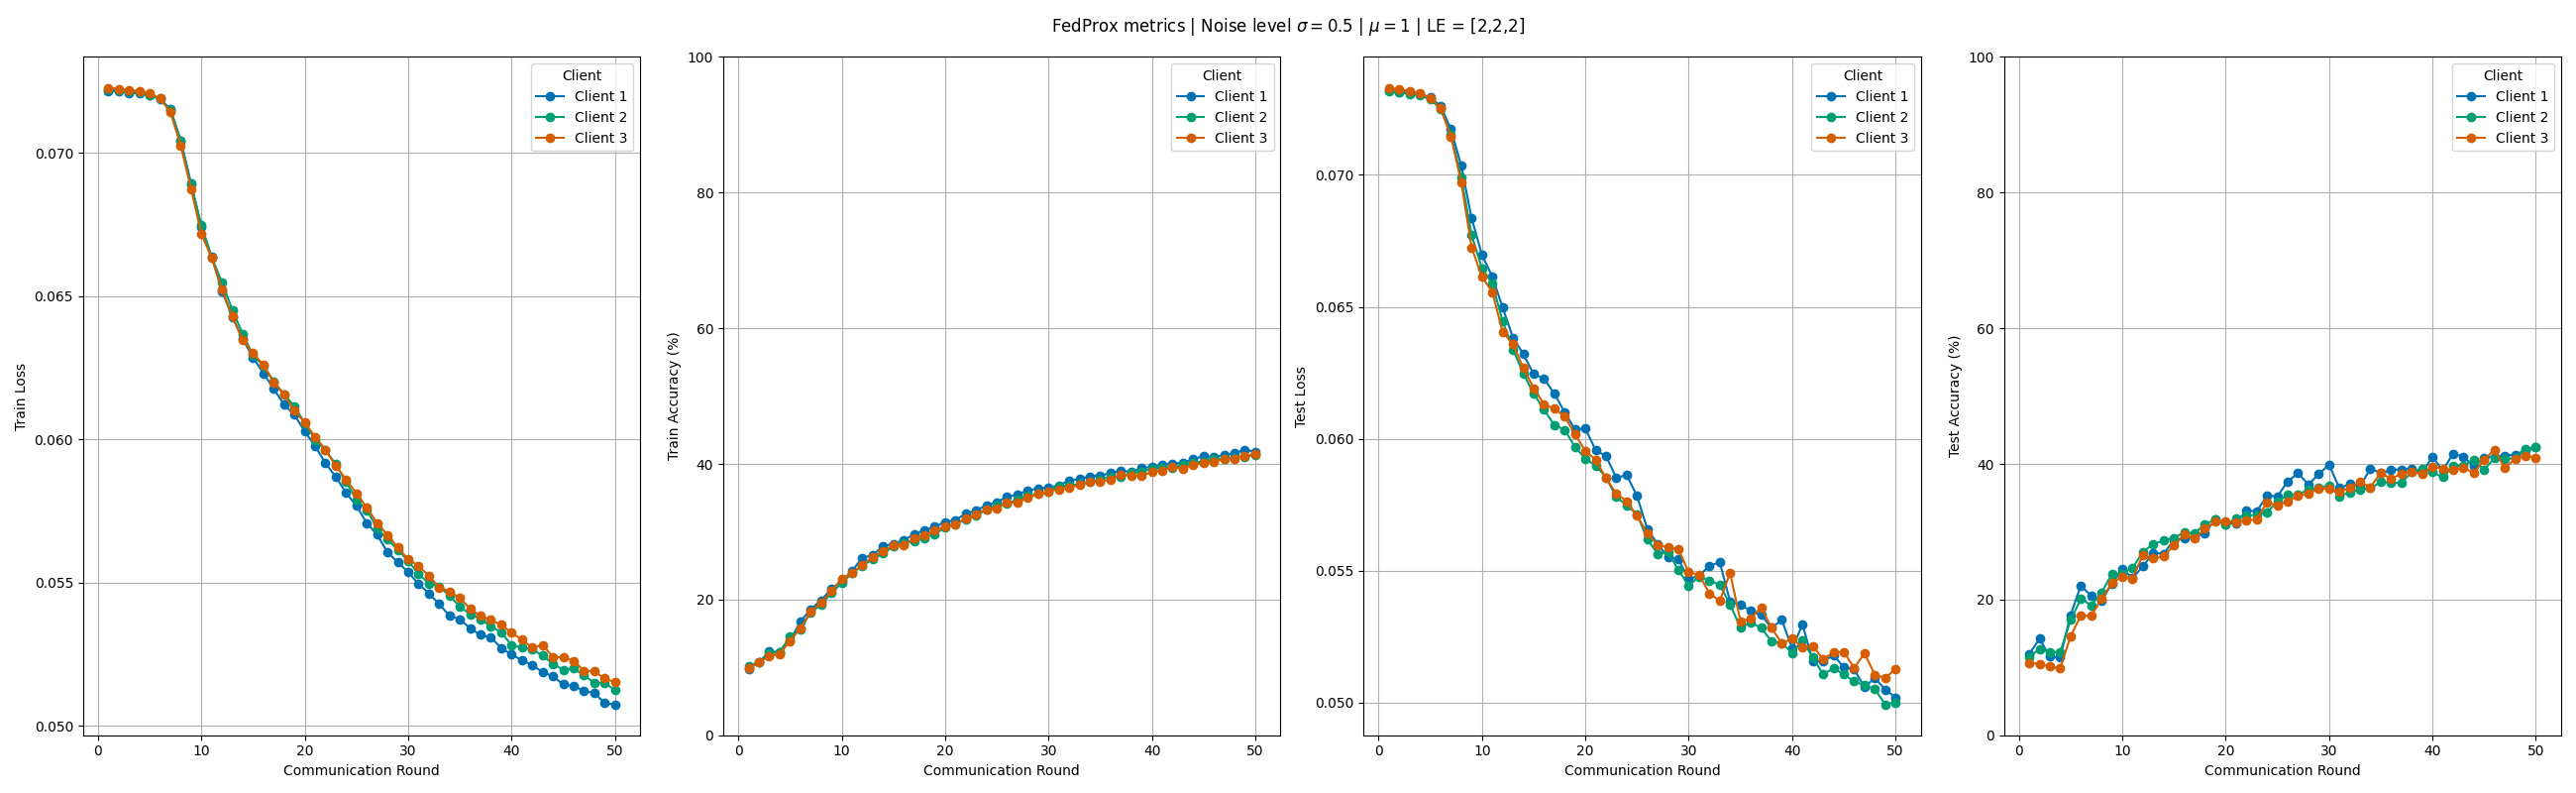
\includegraphics[width=0.8\linewidth]{figures/2-Federated_Learning/FedProx_NoiseLevel_Mu_1.png}
    \end{subfigure}

    \caption{Local metrics for 3 clients in 50 communication rounds using FedProx with a Non-IID setting over the CIFAR10 dataset, $\mu \in \{0.001, 0.01, 0.1, 1\}$. Feature distribution skew using with noise level $\sigma = 0.5$}
    \label{fig:FedProx_Non_IID_NoiseLevel_05}
\end{figure}
